% Source code for my resume in latex, Based on guide from:
% http://www.howtotex.com/general/a-guide-to-building-a-plain-and-simple-latex-cv/


% Preamble
\documentclass[paper=a4, fontsize=11pt]{scrartcl}
 
\usepackage[utf8]{inputenc}
\usepackage[T1]{fontenc}
\usepackage[english,norsk]{babel}
\usepackage{amsmath,amsfonts,amsthm}
\usepackage[pdftex]{graphicx}
\usepackage[svgnames]{xcolor}
\usepackage{geometry}
    \textheight=700px
\usepackage{wrapfig}
\usepackage[colorlinks=true, a4paper=true, pdfstartview=FitV,
            linkcolor=blue, citecolor=blue, urlcolor=blue]{hyperref}

\usepackage{sectsty} 
\definecolor{myred}{RGB}{240, 20, 20}
\sectionfont{
        \color{White}
        \usefont{OT1}{ptm}{m}{n}
        \noindent\colorbox{Grey}
}

% Commands
\newlength{\spacebox} 
\settowidth{\spacebox}{8888888888}

\newlength{\skillbox} 
\settowidth{\skillbox}{8888888888888888}

\newlength{\namebox} 
\settowidth{\namebox}{8888888888888888888888888}

\newcommand{\sepspace}{\vspace*{1em}}

\newcommand{\MyName}[1]{ 
    \Huge \usefont{OT1}{ptm}{m}{n}\noindent#1 
    \par \normalsize \normalfont}

\newcommand{\MySlogan}[1]{
		\Large\usefont{OT1}{ptm}{m}{n}\noindent \textit{#1} % Slogan (optional)
		\par \normalsize \normalfont}

\newcommand{\PersonalEntry}[2]{ 
    \noindent\hangindent=2em\hangafter=0 
    \parbox{\spacebox}{ 
    \textit{#1}} 
    \hspace{1.5em} #2 \par}

 % Same as \PersonalEntry
\newcommand{\SkillsEntry}[2]{						
		\noindent\hangindent=2em\hangafter=0 		% Indentation
		\parbox{\skillbox}{						% Box to align text
		\textit{#1}}								% Entry name (birth, address, etc.)
		\hspace{1.5em} #2 \par}					% Entry value	

\newcommand{\EducationEntry}[4]{ 
    \noindent \textbf{#1} \hfill 
    \colorbox{White}{% 
        \parbox{6em}{% 
        \hfill\color{Black}#2}} \par 
    \noindent \textit{#3} \par 
    \noindent\hangindent=2em\hangafter=0 \small #4 
    \normalsize \par}

\newcommand{\WorkEntry}[4]{						% Same as \EducationEntry
		\noindent \textbf{#1} \hfill 					% Jobname
		\colorbox{White}{\color{Black}#2} \par		% Duration
		\noindent \textit{#3} \par					% Company
		\noindent\hangindent=2em\hangafter=0 \small #4 	% Description
		\normalsize \par}

% Document
\begin{document}

\MyName{Nils Peder Korsveien} 
\MySlogan{Curriculum Vitae}
\sepspace

% Picture
\begin{wrapfigure}{r}{0.3\textwidth} 
    \vspace*{-6em} 
    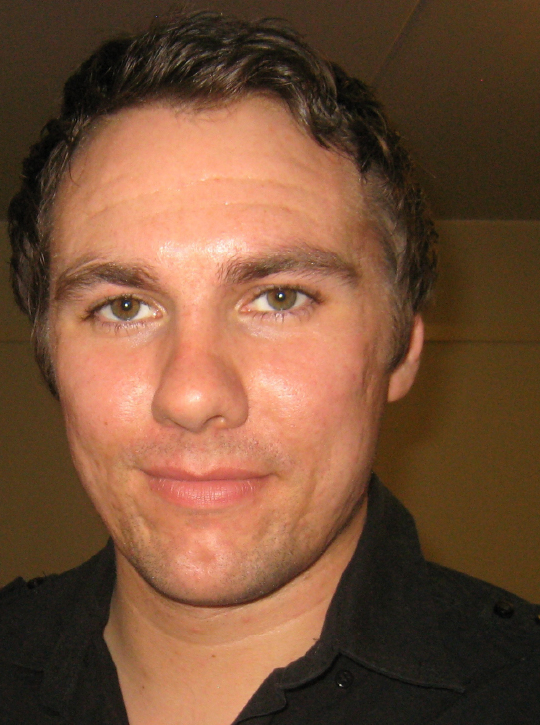
\includegraphics[scale=0.21]{profil} 
    \vspace*{-2em} 
\end{wrapfigure}

\PersonalEntry{}{}
\PersonalEntry{Født}{23.07.1985}
\PersonalEntry{Adresse}{Trimveien 8 H420, 0372 Oslo}
\PersonalEntry{Telefon}{47057184}
\PersonalEntry{Mail} {\href{mailto:nilspk@ulrik.uio.no}{\tt{nilspk@ulrik.uio.no}}}
\PersonalEntry{Web} {\href{http://folk.uio.no/nilspk}{\tt{folk.uio.no/nilspk}}}
\PersonalEntry{Github}{\href{http://github.com/nilspk}{\tt{github.com/nilspk}}}
\sepspace
% \noindent Jeg er en 26 år gammel student som går bachelor i informatikk på
% UiO, samtidig som jeg jobber deltid som kontormedarbeider hos Kredinor.

% dirty, but works
\sepspace
\sepspace
\sepspace
\section*{Utdanning}
\EducationEntry
{Bachelor i Informatikk}
{2009$\rightarrow$}
{UiO}
{Dette er siste semesteret før jeg er ferdig med bachelor graden i
Informatikk. Jeg har lagt ut hvilke emner jeg har tatt på min
hjemmeside.}
\sepspace
\sepspace

\EducationEntry
{Ettårig, Nyere Historie}
{2007-08}
{NTNU}
{Ettårig studie i Trondheim med fag som Stormaktspolitikk, Historiefag,
og Ex.Phil.}
\sepspace
\sepspace

\EducationEntry
{Forkurs for ingeniørfag}
{2007-08}
{HIST}
{Ettårig utdanning jeg tok for å få den nødvendige fordypningen i Matte,
Fysikk og Kjemi som er påkrevd for å søke mer tekniske studiretninger.}
\sepspace
\sepspace

\EducationEntry
{Videregående utdanning}
{2001 - 2004}
{Ringsaker Videregående}
{Jeg studerte 2 år Medier og Kommunikasjon på Ankerskogen VGS på Hamar
,hvor vi drev mye med prosjektarbeid,
før jeg tok Allmennfaglig påbygning på Ringsaker VGS.}
\sepspace
\sepspace
\newpage
\section*{Jobberfaring}
\WorkEntry
{Kontormedarbeider}
{2009$\rightarrow$}
{Kredinor}
{Deltidsansatt på kveldsteam hos Kredinor. Dette er en jobb jeg har hatt
ved siden av studiene i Informatikk. Jeg har jobbet 10 timer i uken
fordelt på to kvelder på hverdager. Å balansere krevende skolearbeid med
deltidsjobb har vært en nyttig og lærerik erfaring.}
\sepspace
\sepspace

\WorkEntry
{Lagermedarbeider}
{2005-08}
{ASKO Hedmark}
{Jobbet som plukker på grossistlager. Dette var en jobb jeg hadde fast
som sommerjobb over noen år, samt en periode på høsten 2008 hvor jeg var
fast ansatt. }
\sepspace
\sepspace

\WorkEntry
{Kassaoperatør}
{2004-05}
{Coop Obs! Rudshøgda}
{Jobb jeg hadde i friåret etter videregående.}
\sepspace

\sepspace
\section*{Kompetanse}
\SkillsEntry{Språk}{Norsk (morsmål)}
\SkillsEntry{}{Engelsk (flytende)}
\sepspace
\SkillsEntry{Programmering}{Java, C, Objective-C, Python, Scheme, SQL, \LaTeX}
\sepspace
\SkillsEntry{OS}{Windows, Mac OS X, Linux}
\sepspace
\SkillsEntry{Annet}{Git, Vim, zsh, screen,  Arduino, Adobe CS, XCode}

\sepspace
\sepspace
\section*{Sideprosjekter}
\WorkEntry
{B.L.I.M.P}
{2011$\rightarrow$}
{En selvflyvende robot!}
{Dette var et prosjekt vi i utgangspunktet startet med i bruksorentert
design, men som var så spennende at vi tok det videre og presenterte det
på Idéfestivalen på Blinderen i September 2011. Video av dette kan sees
her: \href{http://www.bit.ly/ifiblimp}{\tt{youtube-video}}. Prosjektet
har vært ekstremt lærerikt, og planene framover er å ha med roboten vår
på The Gathering, hvor vi har tenkt å promotere instituttet for
Informatikk.}

\sepspace
\sepspace
\section*{Referanse}
Oppgis ved behov.
\end{document}
